\section{Priority Queue} \index{priority queue}

\subsection{Priority Queue ADT}

The priority queue ADT is a data type that stores a collection of items with priorities (keys) that supports the following opeations:

\begin{itemize}
    \item \textsc{Insert}($Q, x$) inserts the element $x$ into the priority queue $Q$.
    \item \textsc{Maximum}($Q$) returns the element of $Q$ with the largest key.
    \item \textsc{Extract-Max}($Q$) removes and returns the element of $q$ with the largest key.
    \item \textsc{Increase-Key}($S,x,k$) increases the value of element $x$'s key into the new value $k$, assuming that $k \geq x$.
\end{itemize}

Priority queue allows us to access the element with largest (if max-priority queue) or smallest (if min-priority queue) more efficiently. It has many applications in computer science, such as: job scheduling in operation systems, bandwith management, or finding minimum spanning tree of a graph, etc.

\subsection{Primitive Implementation Using Linked Lists}

We can have a naive implementation of a priority queue simply using a sorted linked list, which has the following time complexity:
\begin{itemize}
    \item \textsc{Insert}($Q, x$): $\Theta(n)$ in the worst case. We have to linearly search the correct location of insertion.
    \item \textsc{Maximum}($Q$): $\Theta(1)$ by returning the head of the list.
    \item \textsc{Extract-Max}($Q$): $\Theta(1)$ by removing and returning the head of the list.
    \item \textsc{Increase-Key}($S,x,k$): $\Theta(n)$ in the worst case. Need to move element to new location after increase.
\end{itemize}

However, we want to have something that is more efficient than $\Theta(n)$. As it turns out, by putting the elements in a specific way, we can achieve worst-case time complexity of $\Theta(\log n)$ for \textsc{Insert}, \textsc{Extract-Max}, and \textsc{Increase-Key}. Even better, we can show that the amortized complexity of \textsc{Insert} is $\Theta(1)$ and \textsc{Extract-Max} is $\Theta(\log n)$.

\section{Heap} \index{heap}

\subsection{Types of Binary Trees}

Before starting to formally define heaps, let's review some definitions about binary trees. 

\begin{definition}[Full Binary Tree] \index{full binary tree}
    A full binary tree (sometimes proper binary tree or 2-tree) is a tree in which every node other than the leaves has two children. 
\end{definition}

\begin{definition}[Complete Binary Tree] \index{complete binary tree}
    A complete binary tree is a binary tree in which every level, except possibly the last, is completely filled, and all nodes are as far left as possible.

    Importantly, a complete binary tree with $n$ nodes has $\left\lfloor n / 2 \right\rfloor$ internal nodes (nodes that are not leaves).
\end{definition}

\begin{definition}[Perfect Binary Tree] \index{perfect binary tree}
    A perfect binary tree is a binary tree in which all interior nodes have two children and all leaves have the same depth or same level.
\end{definition}

\begin{figure}[h!]
    \centering
    \tikzset{every tree node/.style={minimum width=1em,draw,circle},
         blank/.style={draw=none},
         edge from parent/.style=
         {draw,edge from parent path={(\tikzparentnode) -- (\tikzchildnode)}},
         level distance=2em}
    \vcenteredhbox{
        \begin{tikzpicture}
            \Tree [.{} [.{} {} [.{} {} {} ] ]
            {} ]
        \end{tikzpicture}
    }
    \hfil
    \vcenteredhbox{
        \begin{tikzpicture}
            \Tree [.{} [.{} {} {} ]
            [.{} {} {} ] ]
        \end{tikzpicture}
    }
    \hfil
    \vcenteredhbox{
        \begin{tikzpicture}
            \Tree [.{} [.{} {} {} ]
            [.{} {} \edge[blank]; \node[blank]{}; ] ]
        \end{tikzpicture}
    }
    \caption{From left to right: full binary tree, complete binary tree, perfect binary tree.}
\end{figure}

Conveniently, a complete binary tree can be represented as an array.

\begin{figure}[htbp]
    \centering
    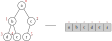
\includegraphics[width=0.6\linewidth]{figures/heap_as_arr.pdf}
    \caption{A complete binary tree and its corresponding array representation}
\end{figure}

Assuming that we index from 0, we can compute the indices of each node's parent, left, and right child.

\textsc{Parent}(i) = $\left\lfloor (i-1) / 2 \right\rfloor$ \\
\textsc{Left}(i) = $(2i)+1$ \\
\textsc{Right}(i) = $(2i)+2$

If we index from 1, the indices are calculated as follows:

\textsc{Parent}(i) = $\left\lfloor i / 2 \right\rfloor$ \\
\textsc{Left}(i) = $2i$ \\
\textsc{Right}(i) = $2i+1$

\subsection{Heap Property}

Then, we can define a max-heap as a complete binary tree with the max-heap property.

\begin{definition}[Max-heap Property] \index{max-heap property} \index{max-heap}
    In a max-heap represented by the array $A$ , the max-heap property is that for every node $i$ other than the root,
    \[
        A[\textsc{Parent}(i)] \geq A[i]
    .\]
    that is, the value of a node is at most the value of its parent.
\end{definition}

The max-heap property guarantees that the largest element in a heap is always stored at its root.

For our heap implementation, we will include the following operations: \proc{Insert}, \proc{Maximum}, \proc{Extract-Max}, \proc{Increase-Key}, \proc{Max-Heapify}, \proc{Build-Max-Heap}. The first few operations allow us to use heap to implement the priority queue ADT, and in addition to those, \proc{Build-Max-Heap} allows us to produce a max-heap from an unordered array.

\section{Maintaining the Heap Property}

Given an array $A$ and index $i$, \proc{Max-Heapify} will correct a single violation of the max-heap property in the subtree with $i$ as its root. To implement \proc{Max-Heapify}, we use a technique called ``trickle down''.

First, assume that the trees rooted at $\proc{Left}(i)$ and $\proc{Right}(i)$ are max-heaps. If element $A[i]$ violates the max-heap property, we correct thie violation by ``trickling'' element $A[i]$ down the tree until it reaches the correct position. By doing so, we can make the subtree rooted at index $i$ a max-heap. In every trickle-down step, swap $A[i]$ with its largest child.

\begin{codebox}
    \Procname{$\proc{Max-Heapify}(A,i)$}
    \li $l = \proc{Left}(i)$
    \li $r = \proc{Right}(i)$ 
    \li \If $l \leq A.heap-size$ and $A[l] > A[i]$
    \li \Then $largest = l$
    \li \Else $largest = i$
    \End
    \li \If $r \leq A.heap-size$ and $A[r] > A[largest]$ 
    \li \Then $largest = r$
    \End
    \li \If $largest \neq i$
    \li \Then exchange $A[i]$ with $A[largest]$
    \li       $\proc{Max-Heapify}(A,largest)$
    \End 
\end{codebox}

\subsection{Correctness of \proc{Max-Heapify}}

\subsection{Running Time of \proc{Max-Heapify}}

\section{Inserting Into Max-Heap}

To insert into a max-heap while maintaining the heap property, we use a similar technique. We first append the new element to the end of the heap. The new element will become the right-most leaf at the last level. Then, we check if the element is already at the right position. If not, we ``bubble'' the element up the tree, until it reaches the correct position.

\section{Build Heap From Unsorted Array}

\begin{codebox}
    \Procname{$\proc{Build-Max-Heap}(A)$}
    \li $A.heapsize = A.length$
    \li \For $i = \left\lfloor A.length / 2 \right\rfloor$ \textbf{downto} 1
    \li \Then $\proc{Max-Heapify}(A,i)$
    \End
\end{codebox}


The reason we start calling \proc{Max-Heapify} at $\left\lfloor A.length / 2 \right\rfloor$ is because elements beyond that $A[n / 2+1, \cdots, n]$ are all leaves of the tree. Recall that for a complete binary tree with $n$ nodes, there are only $\left\lfloor n / 2 \right\rfloor$ internal nodes.

\subsection{Running Time of \proc{Build-Max-Heap}}

Each call of \proc{Max-Heapify} takes $O(\log n)$ time, and \proc{Build-Max-Heap} calls \proc{Max-Heapify} $O(n)$ times. Thus, the running time of \proc{Build-Max-Heap} is $O(n \log n)$. However, this upper bound is not tight. We will prove a tighter upper bound of $O(n)$.

{
    \setlength\columnsep{4em}
    \begin{multicols}{2}
        
        Note that \proc{Max-Heapify} takes $O(1)$ time for nodes tthat are one level above the leaves, and in general, it takes $O(k)$ for nodes that are $k$ levels above the leaves.
        We have $n / 4$ nodes at level 1, $n / 8$ at level 2, etc. At the root level, which is $\log_2 n$ levels above the leaves, we have only 1 node.

        \includegraphics[width=\linewidth]{figures/build_max_heap.pdf}
    \end{multicols}
}

More generally, a heap with $n$ nodes has a height of $\left\lfloor \log_2 n \right\rfloor$ and at most $\left\lceil n / 2^{h+1} \right\rceil $ nodes at any height $h$. Hence, the total cost of \proc{Build-Max-Heap} can be written as
\[
\sum_{h=0}^{\left\lfloor \log_2 n \right\rfloor} \left\lceil \frac{n}{2^{h+1}} \right\rceil O(h) = O \left( n \sum_{h=0}^{\log_2 n} \frac{h}{2^h} \right)
.\]
The last summation is bounded by a constant, namely
\[
\sum_{h=0}^{\log_2 n} \frac{h}{2^h} \leq \sum_{h=0}^{\infty} \frac{h}{2^h} = 2 = O(1)
.\]
Thus,
\[
O \left( n \sum_{h=0}^{\log_2 n} \frac{h}{2^h} \right) = O(n) O(1) = O(n)
.\]

\section{Heapsort}

\begin{codebox}
    \Procname{$\proc{Heapsort}(A)$}
    \li \For $i = A.length$ \textbf{downto} 2
    \li \Then exchange $A[1]$ with $A[i]$
    \li $A.heapsize = A.heapsize - 1$
    \li $\proc{Max-Heapify}(A,1)$
    \End 
\end{codebox}